\subsection{Application Server}\label{sec:impl-as}

% TODO: Update if something changes
As we previously said in Section \ref{sec:sol-des-as}, our Phoenix Application
Server is composed of two sub-applications, namely \texttt{Domain} and
\texttt{Interface}.

\subsubsection{Domain}

\texttt{Domain} can be roughly seen as a supervision tree, which at the top has
the root \texttt{Domain} module itself. This module supervises $O(k * m)$
modules, where $k$ is the number of cities and $m$ the number of districts per
city.

In Figure \ref{fig:impl-as-domain} we can see a visual representation of this
tree: even if in the picture \texttt{DistrictInfo} GenServers (i.e., the
per-district trackers) are grouped by city (e.g., $A$ in the drawing), the
supervision tree has an actual depth of 1\footnote{that's why there is a
dotted line around each \texttt{DistrictInfo}}.
We could also have placed one intermediate supervisors for each city, but
there was no special need to do it.

Always in Figure \ref{fig:impl-as-domain}, we can notice that there is another
GenServer supervised other than the \texttt{DistrictInfo}s: this is the
\texttt{Loader} module, which is responsible for loading static information in
the district trackers when our Application Server starts. We chose to employ a
supervised GenServer (that can be also viewed as an Elixir process) and not a
task because we use the \texttt{Loader} module at runtime too, when a
simulation ends and we want to reset a district tracker to its initial
configuration values.

\begin{figure}[H]
  \centering
  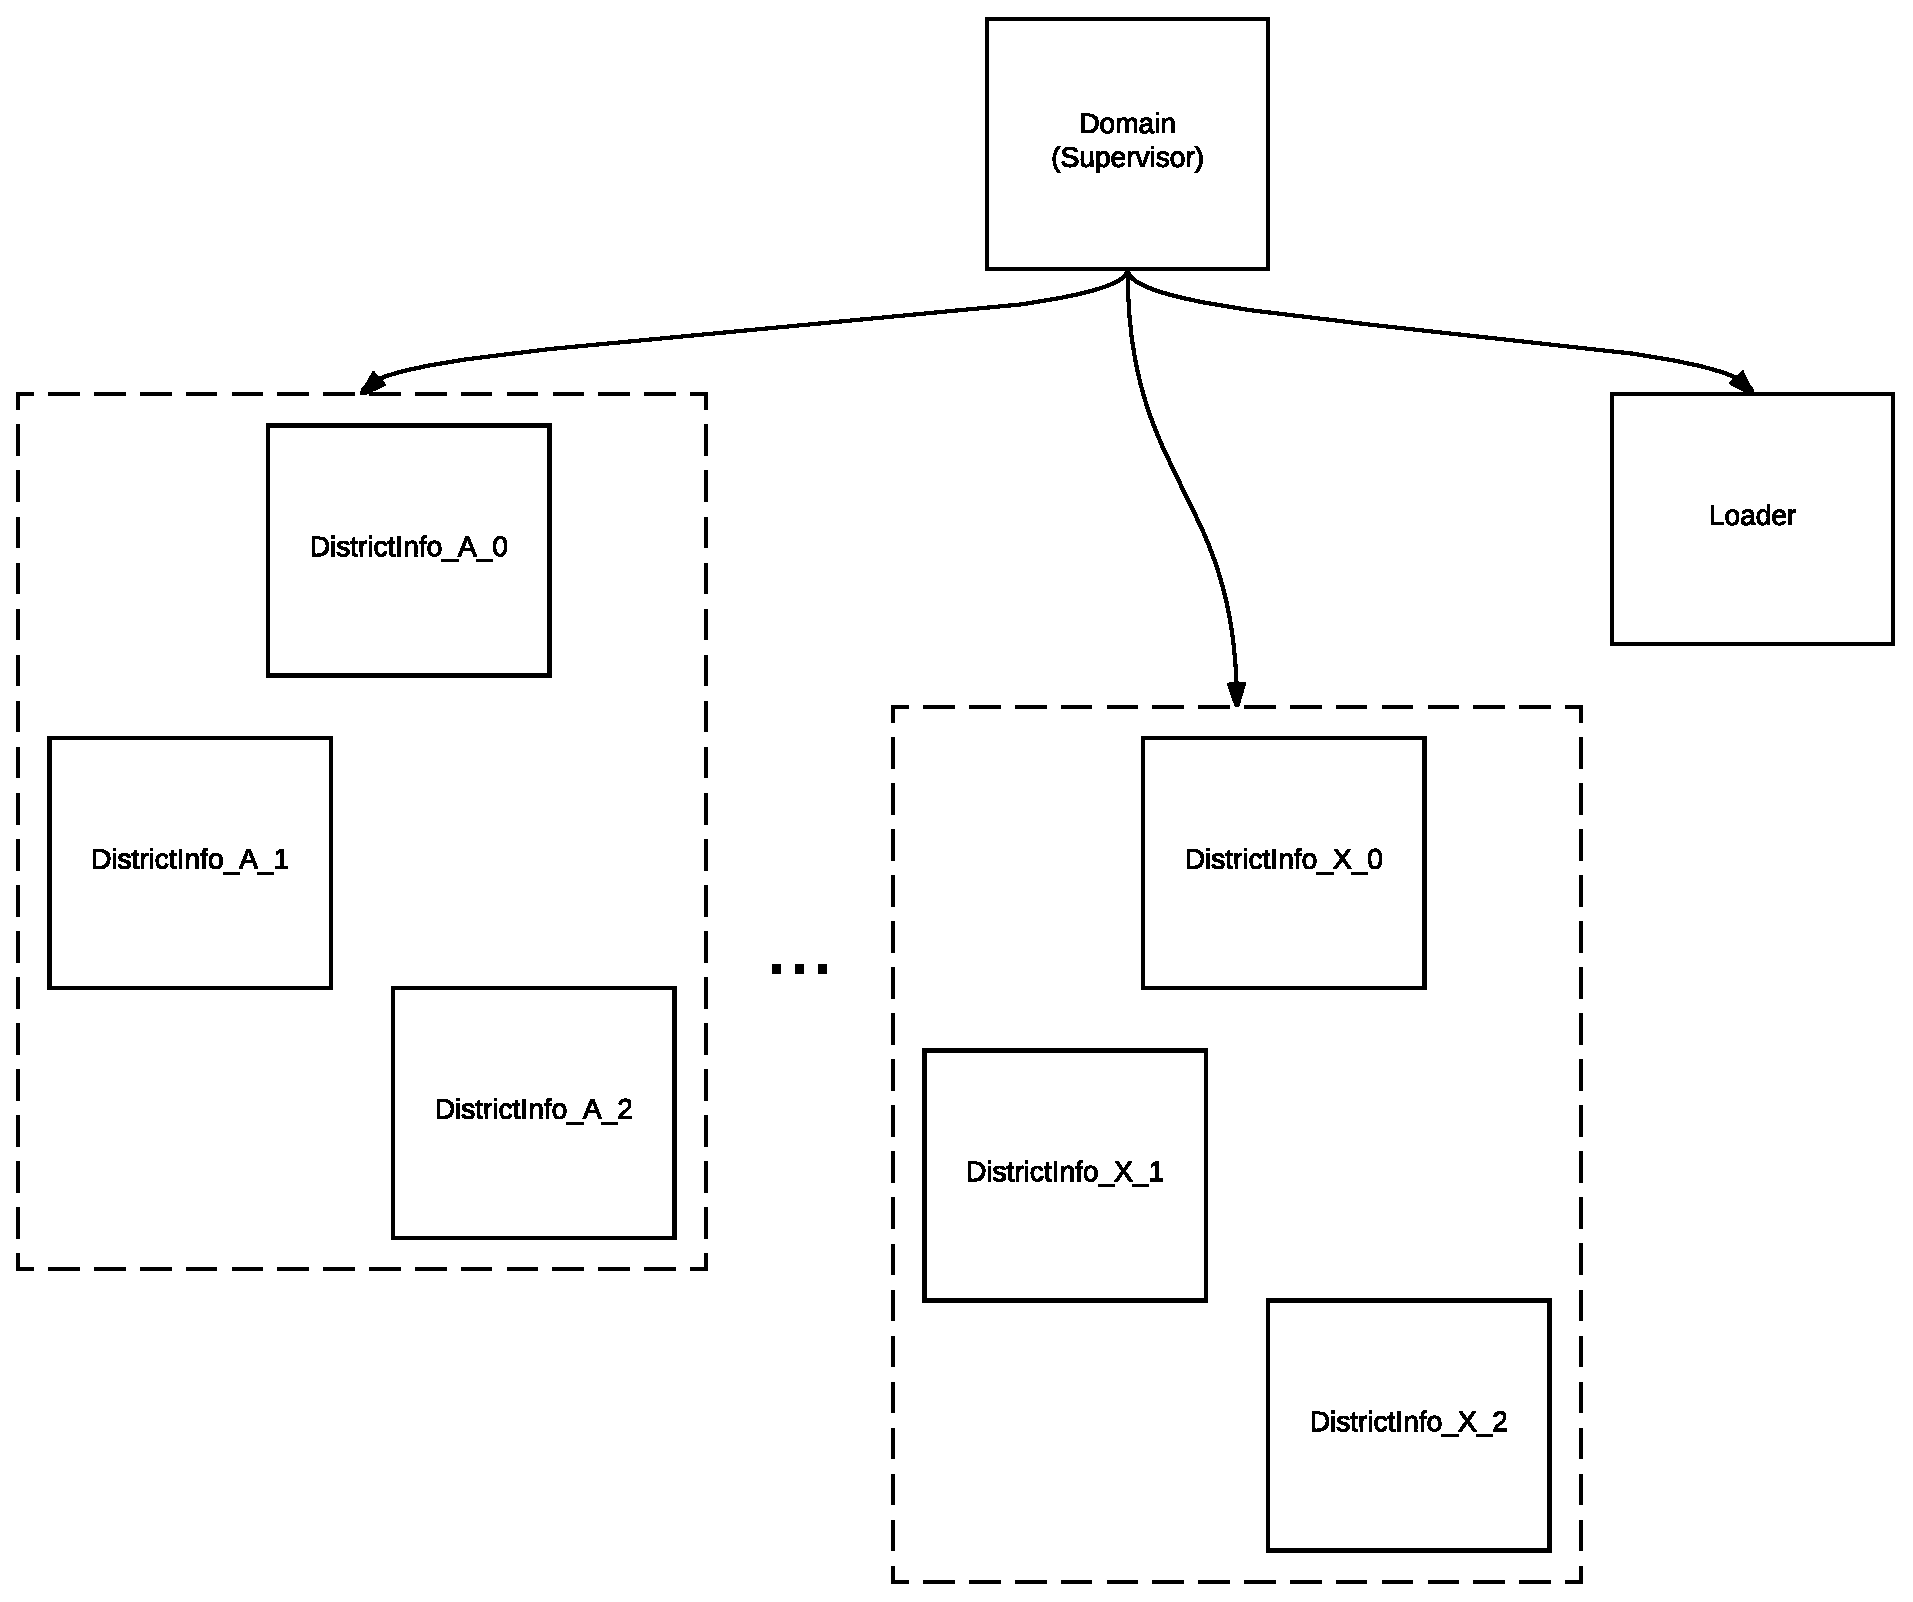
\includegraphics[width=\columnwidth]{images/implementation/as-domain.eps}
  \caption{Domain supervision tree}
  \label{fig:impl-as-domain}
\end{figure}

\subsubsection{Interface}

% TODO: Write...

\begin{figure}[H]
  \centering
  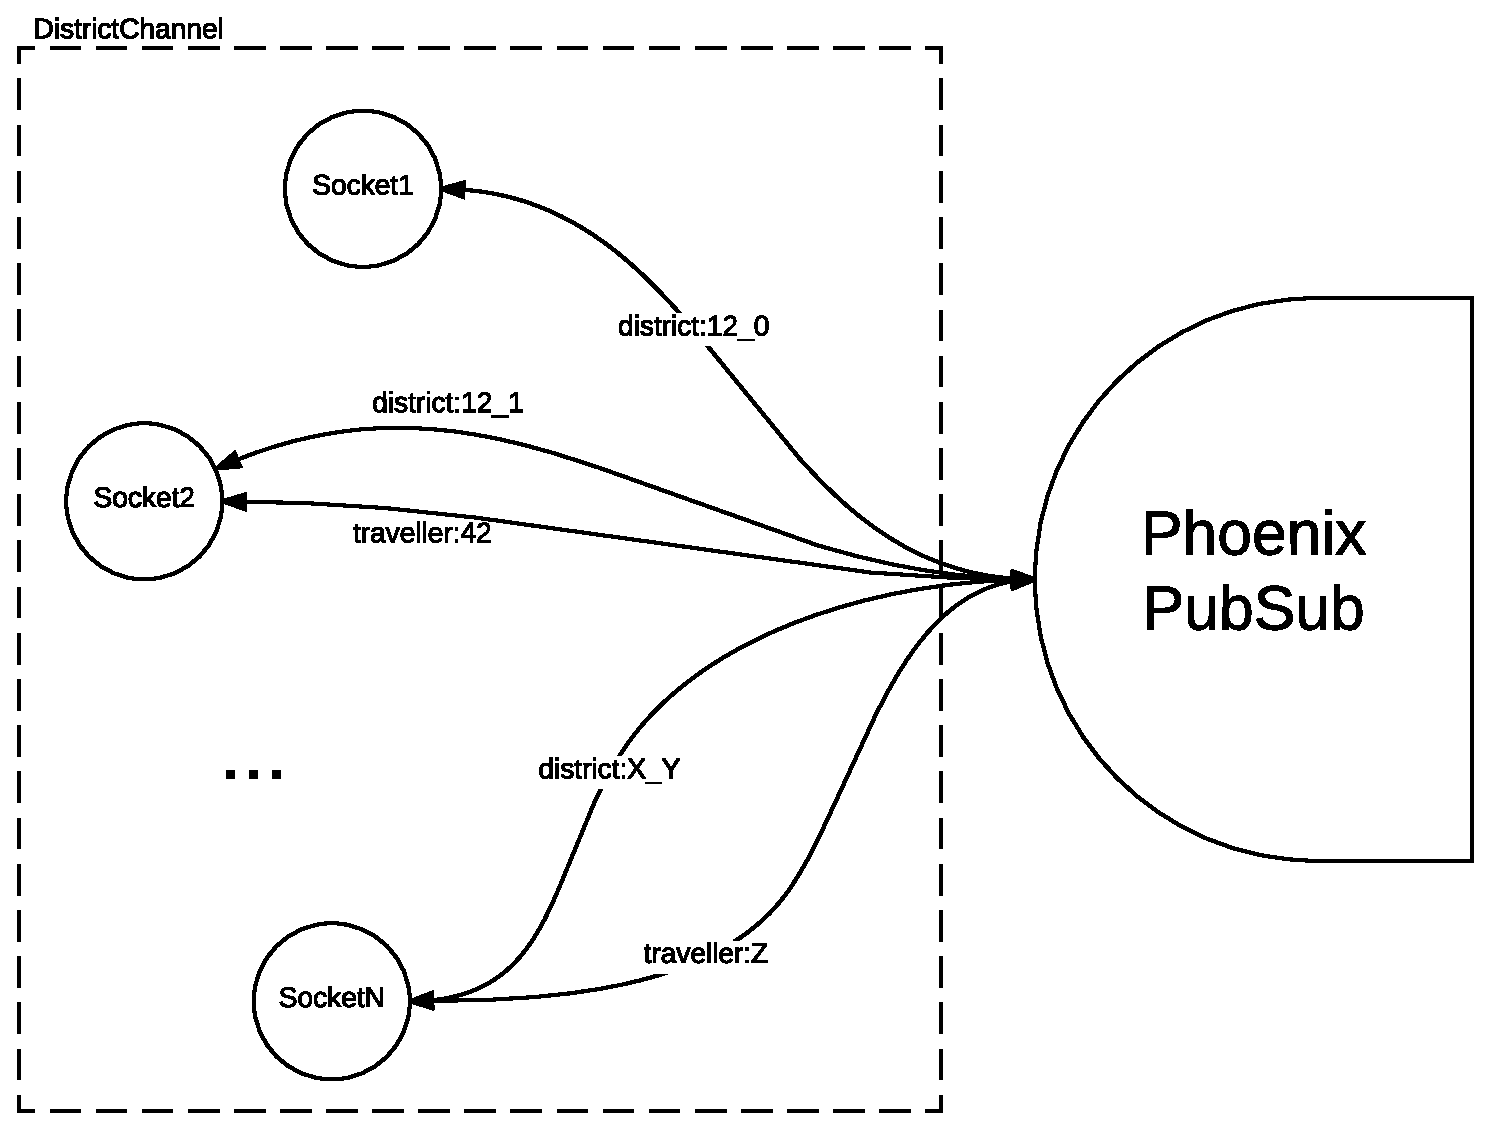
\includegraphics[width=\columnwidth]{images/implementation/as-chan-pubsub.eps}
  \caption{\texttt{DistrictChannel} pub/sub system}
  \label{fig:impl-as-pubsub}
\end{figure}
